\Chapter{ETUDE DU SAUT D'UNE ROUE CYR}\label{sec:Theme1}
\begin{table}[htbp]
  \centering
  \caption{Constantes et variables des modèle analytiques}
  \begin{tabular}{|c|l|}
    \hline \rowcolor[gray]{0.8}\color{black}
    Symbole         & Description\\
    $A$           & Aire de la section\\
   
    $E$           & Module d'Young du matériau\\
    $E_{p,g}$          & Energie potentielle gravitationnelle\\
    $E_{tot}$          & Energie mécanique totale\\
    $F$             & Force de compression appliquée à la roue\\
    $g$     & Accélération gravitationnelle\\
    $H_{max}$          & Hauteur de saut maximale\\
    $I$           & Moment quadratique de la section\\
    $k$             & raideur équivalente de la roue\\
    $m_r$          & Masse de la roue\\
    
    $R$       & Rayon médian de la roue\\
    $r_1$ & Rayon interne de section pour une section circulaire\\
    $r_2$             & rayon externe de section pour une section circulaire\\
    $\rho$           & Masse volumique du matériau\\ \hline
  \end{tabular}
  \label{tab:Definitions}
\end{table}


\section{Etude théorique}
\subsection{Description du mouvement}
La roue Cyr est comprimée par une force $F$ exercée selon l'axe de son diamètre puis relâchée. Une partie de l'énergie de déformation élastique est transformée en saut. On notera $H_{max}$ la hauteur correspondant à l'énergie potentielle par laquelle s'élève le centre de gravité de la roue de sa position au repos à sa hauteur maximale.


\subsubsection{Hypothèses}
\begin{itemize}
    \item On considère que le support contre lequel la roue est comprimée est parfaitement rigide.
    \item On néglige la force de traînée de l'air.
    \item La répartition des masses est idéalisée
\end{itemize}

\subsubsection{Modèle deux degrés de liberté}
On modélise la roue Cyr par deux masses ponctuelles égales $m_r/2$ reliées par un ressort de longueur à vide $2R$, où $R$ correspond au rayon médian de la roue, et de rigidité $k$. \\
La rigidité équivalente de la roue est donnée par \cite{yangkim}:
\begin{equation}
    k=\frac{4\pi EI}{(\pi^2 -8)R^3},
    \label{eq:0}
\end{equation}

où $E$ est le module d'Young et $I$ est le moment moment quadratique de la section de la roue.

\\
 Les positions des masses sont reperées par les ordonnées $y_1(t)$ et $y_2(t)$.

\begin{figure}[htb]
\centering

%% Creator: Inkscape inkscape 0.92.2, www.inkscape.org
%% PDF/EPS/PS + LaTeX output extension by Johan Engelen, 2010
%% Accompanies image file 'repos2.eps' (pdf, eps, ps)
%%
%% To include the image in your LaTeX document, write
%%   \input{<filename>.pdf_tex}
%%  instead of
%%   \includegraphics{<filename>.pdf}
%% To scale the image, write
%%   \def\svgwidth{<desired width>}
%%   \input{<filename>.pdf_tex}
%%  instead of
%%   \includegraphics[width=<desired width>]{<filename>.pdf}
%%
%% Images with a different path to the parent latex file can
%% be accessed with the `import' package (which may need to be
%% installed) using
%%   \usepackage{import}
%% in the preamble, and then including the image with
%%   \import{<path to file>}{<filename>.pdf_tex}
%% Alternatively, one can specify
%%   \graphicspath{{<path to file>/}}
%% 
%% For more information, please see info/svg-inkscape on CTAN:
%%   http://tug.ctan.org/tex-archive/info/svg-inkscape
%%
\begingroup%
  \makeatletter%
  \providecommand\color[2][]{%
    \errmessage{(Inkscape) Color is used for the text in Inkscape, but the package 'color.sty' is not loaded}%
    \renewcommand\color[2][]{}%
  }%
  \providecommand\transparent[1]{%
    \errmessage{(Inkscape) Transparency is used (non-zero) for the text in Inkscape, but the package 'transparent.sty' is not loaded}%
    \renewcommand\transparent[1]{}%
  }%
  \providecommand\rotatebox[2]{#2}%
  \ifx\svgwidth\undefined%
    \setlength{\unitlength}{337.82993867bp}%
    \ifx\svgscale\undefined%
      \relax%
    \else%
      \setlength{\unitlength}{\unitlength * \real{\svgscale}}%
    \fi%
  \else%
    \setlength{\unitlength}{\svgwidth}%
  \fi%
  \global\let\svgwidth\undefined%
  \global\let\svgscale\undefined%
  \makeatother%
  \begin{picture}(1,0.62816437)%
    \put(0,0){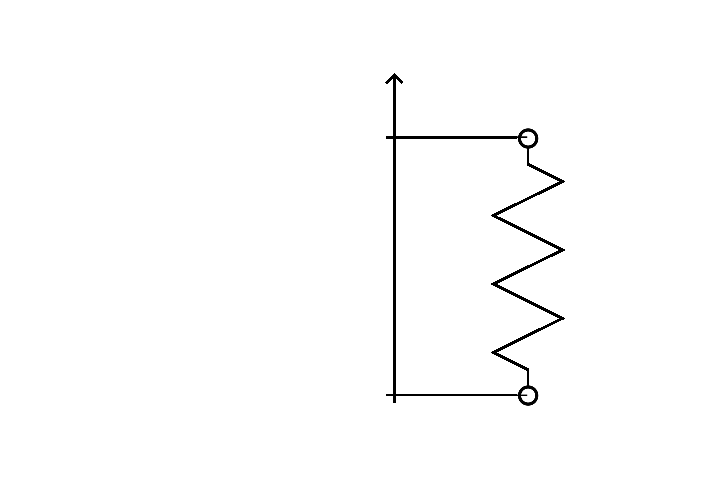
\includegraphics[width=\unitlength]{images_2ddl/repos2.eps}}%
    \put(0.53610169,0.57938811){\color[rgb]{0,0,0}\makebox(0,0)[lb]{\smash{$y$}}}%
    \put(0.29,0.46){\color[rgb]{0,0,0}\makebox(0,0)[lb]{\smash{$y_1=2R-\dfrac{m_r g}{2k}$}}}%
    \put(0.42,0.09){\color[rgb]{0,0,0}\makebox(0,0)[lb]{\smash{$y_2=0$}}}%
    \put(0.62490379,0.2696811){\color[rgb]{0,0,0}\makebox(0,0)[lb]{\smash{$k$}}}%
    \put(0.7581069,0.49168631){\color[rgb]{0,0,0}\makebox(0,0)[lb]{\smash{$\dfrac{m_r}{2}$}}}%
    \put(0.78030738,0.0698765){\color[rgb]{0,0,0}\makebox(0,0)[lb]{\smash{$\dfrac{m_r}{2}$}}}%
  \end{picture}%
\endgroup%

\caption{Système au repos. Le ressort de longueur à vide $2R$ et de raideur $k$ est écrasé par le poids de la masse supérieure.}
\label{fig:repos}
\end{figure}

\subsection{Mise en équations}

On note $t=-t_0$ le moment auquel on relâche le ressort, $t=0$ le moment auquel la masse inférieure quitte le sol et $t_f$ le moment auquel le centre de gravité du système atteint sa hauteur maximale.
\\

\begin{figure}[h]

\def\svgwidth{400}
%% Creator: Inkscape inkscape 0.92.2, www.inkscape.org
%% PDF/EPS/PS + LaTeX output extension by Johan Engelen, 2010
%% Accompanies image file 'saut1.eps' (pdf, eps, ps)
%%
%% To include the image in your LaTeX document, write
%%   \input{<filename>.pdf_tex}
%%  instead of
%%   \includegraphics{<filename>.pdf}
%% To scale the image, write
%%   \def\svgwidth{<desired width>}
%%   \input{<filename>.pdf_tex}
%%  instead of
%%   \includegraphics[width=<desired width>]{<filename>.pdf}
%%
%% Images with a different path to the parent latex file can
%% be accessed with the `import' package (which may need to be
%% installed) using
%%   \usepackage{import}
%% in the preamble, and then including the image with
%%   \import{<path to file>}{<filename>.pdf_tex}
%% Alternatively, one can specify
%%   \graphicspath{{<path to file>/}}
%% 
%% For more information, please see info/svg-inkscape on CTAN:
%%   http://tug.ctan.org/tex-archive/info/svg-inkscape
%%
\begingroup%
  \makeatletter%
  \providecommand\color[2][]{%
    \errmessage{(Inkscape) Color is used for the text in Inkscape, but the package 'color.sty' is not loaded}%
    \renewcommand\color[2][]{}%
  }%
  \providecommand\transparent[1]{%
    \errmessage{(Inkscape) Transparency is used (non-zero) for the text in Inkscape, but the package 'transparent.sty' is not loaded}%
    \renewcommand\transparent[1]{}%
  }%
  \providecommand\rotatebox[2]{#2}%
  \ifx\svgwidth\undefined%
    \setlength{\unitlength}{458.93788937bp}%
    \ifx\svgscale\undefined%
      \relax%
    \else%
      \setlength{\unitlength}{\unitlength * \real{\svgscale}}%
    \fi%
  \else%
    \setlength{\unitlength}{\svgwidth}%
  \fi%
  \global\let\svgwidth\undefined%
  \global\let\svgscale\undefined%
  \makeatother%
  \begin{picture}(1,0.55996795)%
    \put(0,0){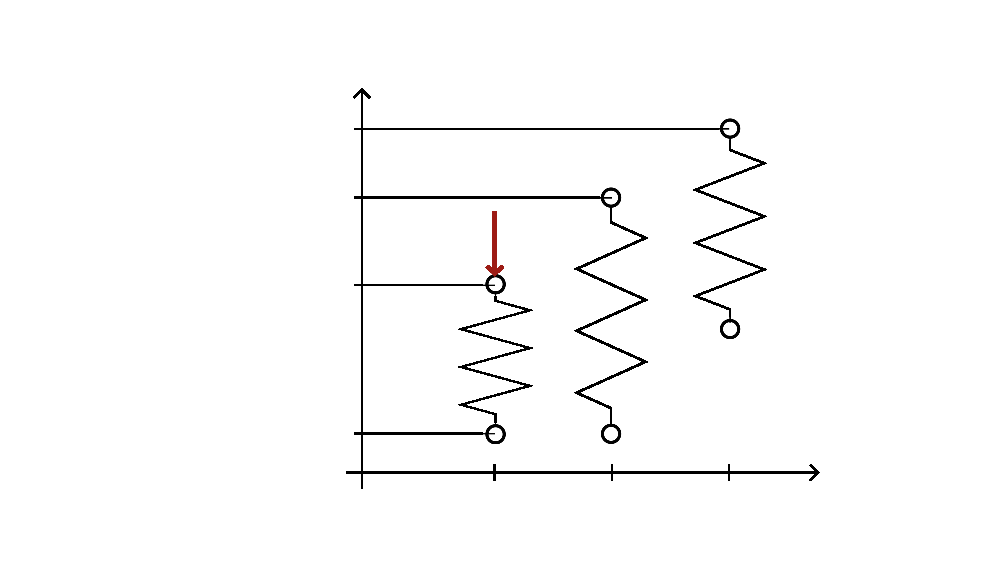
\includegraphics[width=\unitlength]{images_2ddl/saut1.eps}}%
    \put(0.35332121,0.50424636){\color[rgb]{0,0,0}\makebox(0,0)[lb]{\smash{$y$}}}%
    \put(0.85079889,0.07843695){\color[rgb]{0,0,0}\makebox(0,0)[lb]{\smash{$t$}}}%
    \put(0.44868441,0.03798154){\color[rgb]{0,0,0}\makebox(0,0)[lb]{\smash{$t<-t_0$}}}%
    \put(0.59510438,0.04003324){\color[rgb]{0,0,0}\makebox(0,0)[lb]{\smash{$t=0$}}}%
    \put(0.71660123,0.03978188){\color[rgb]{0,0,0}\makebox(0,0)[lb]{\smash{$t=t_f$}}}%
    \put(0.31206609,0.11596114){\color[rgb]{0,0,0}\makebox(0,0)[lb]{\smash{$0$}}}%
    \put(0.12576987,0.27218246){\color[rgb]{0,0,0}\makebox(0,0)[lb]{\smash{$2R-\dfrac{F}{k}-\dfrac{m_r g}{2k}$}}}%
    \put(0.19576987,0.36438468){\color[rgb]{0,0,0}\makebox(0,0)[lb]{\smash{$2R+\dfrac{m_r g}{2k}$}}}%
    \put(0.25429501,0.44056847){\color[rgb]{0,0,0}\makebox(0,0)[lb]{\smash{$y_{1,max}$}}}%
    \put(0.51238222,0.3284082){\color[rgb]{0.61568627,0.10588235,0.07843137}\makebox(0,0)[lb]{\smash{$F$}}}%
  \end{picture}%
\endgroup%


\caption{Saut du système. Pour $t<-t_0$, le système est écrasé par une force F. Il est relâche à $t=-t_0$, et la masse inférieure quitte le sol à $t=0$. Le centre de gravité du système atteint sa hauteur maximale pour $t=t_f$}
\label{fig:saut}
\end{figure}

$$
$$
$$
$$


Avant que la masse inférieure ne quitte le sol ($y_2=0$), la masse supérieure est soumise à deux forces de directions confondues avec l'axe du ressort: son propre poids de norme $-\frac{m_r g}{2}$, et la force élastique de norme $-k(y_1-2R)$. Son mouvement est régi par:

\begin{equation}
    \frac{m_r}{2}\frac{d^2y_1}{dt^2}+k(y_1-2R)+\frac{m_r}{2}g=0,
  \label{eq:1}
\end{equation}
pour $-t_0<t<0$,\\

avec les condition initiales:

\begin{align}
    &y_1(-t_0)=2R-\frac{F}{k}-\frac{m_r g}{2k} \nonumber\\
    &\frac{dy_1}{dt}(-t_0)=0
\label{eq:1i}
\end{align}


et où $g$ est l'accélération gravitationnelle. \\
  
A partir du moment où la masse inférieure quitte le sol, la force qui lui est transmise par le ressort devient suffisante pour prendre le dessus sur la gravité: $\frac{m_r g}{2}=k(y_1-2R)$  et la position des deux masses est donnée par:

\begin{align}
    \frac{m_r}{2}\frac{d^2y_1}{dt^2}+k(y_1-y_2-2R)+\frac{m_r}{2}g&=0 \nonumber\\
    \frac{m_r}{2}\frac{d^2y_2}{dt^2}+k(y_2-y_1+2R)+\frac{m_r}{2}g&=0,
  \label{eq:3}
\end{align}

pour $0<t<t_f$,\\
avec les conditions initiales: 

\begin{align}
    y_1(0)=&2R+\frac{m_r g}{2k} & \frac{d y_1}{dt}(0)=&v_{10}\nonumber\\
    y_2(0)=&0 & \frac{d y2}{dt}(0)=&0
  \label{eq:4}
\end{align}    
    


\begin{figure}[htb]
\centering
\def\svgwidth{350}
%% Creator: Inkscape inkscape 0.92.2, www.inkscape.org
%% PDF/EPS/PS + LaTeX output extension by Johan Engelen, 2010
%% Accompanies image file 'sautp.eps' (pdf, eps, ps)
%%
%% To include the image in your LaTeX document, write
%%   \input{<filename>.pdf_tex}
%%  instead of
%%   \includegraphics{<filename>.pdf}
%% To scale the image, write
%%   \def\svgwidth{<desired width>}
%%   \input{<filename>.pdf_tex}
%%  instead of
%%   \includegraphics[width=<desired width>]{<filename>.pdf}
%%
%% Images with a different path to the parent latex file can
%% be accessed with the `import' package (which may need to be
%% installed) using
%%   \usepackage{import}
%% in the preamble, and then including the image with
%%   \import{<path to file>}{<filename>.pdf_tex}
%% Alternatively, one can specify
%%   \graphicspath{{<path to file>/}}
%% 
%% For more information, please see info/svg-inkscape on CTAN:
%%   http://tug.ctan.org/tex-archive/info/svg-inkscape
%%
\begingroup%
  \makeatletter%
  \providecommand\color[2][]{%
    \errmessage{(Inkscape) Color is used for the text in Inkscape, but the package 'color.sty' is not loaded}%
    \renewcommand\color[2][]{}%
  }%
  \providecommand\transparent[1]{%
    \errmessage{(Inkscape) Transparency is used (non-zero) for the text in Inkscape, but the package 'transparent.sty' is not loaded}%
    \renewcommand\transparent[1]{}%
  }%
  \providecommand\rotatebox[2]{#2}%
  \ifx\svgwidth\undefined%
    \setlength{\unitlength}{431.9999892bp}%
    \ifx\svgscale\undefined%
      \relax%
    \else%
      \setlength{\unitlength}{\unitlength * \real{\svgscale}}%
    \fi%
  \else%
    \setlength{\unitlength}{\svgwidth}%
  \fi%
  \global\let\svgwidth\undefined%
  \global\let\svgscale\undefined%
  \makeatother%
  \begin{picture}(1,0.83333334)%
    \put(0,0){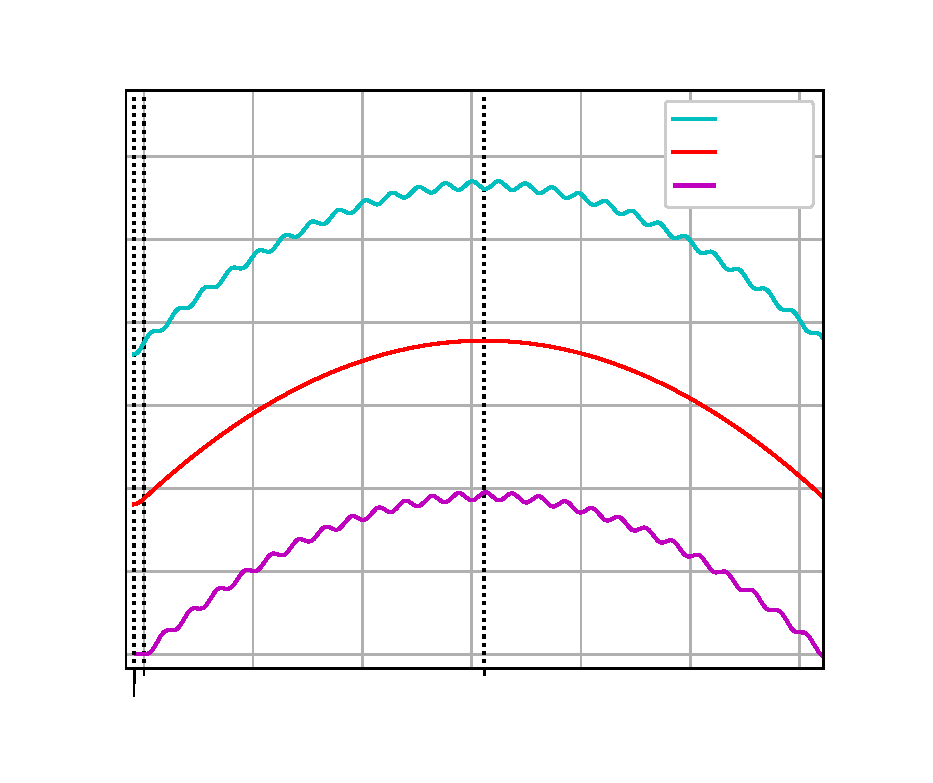
\includegraphics[width=\unitlength]{images_2ddl/sautp.eps}}%
    \put(0.79467593,0.71228239){\color[rgb]{0,0,0}\makebox(0,0)[lb]{\smash{$y_1(t)$}}}%
    \put(0.79467593,0.67524535){\color[rgb]{0,0,0}\makebox(0,0)[lb]{\smash{$y_{cdg}(t)$}}}%
    \put(0.79467593,0.63820832){\color[rgb]{0,0,0}\makebox(0,0)[lb]{\smash{$y_2(t)$}}}%
    \put(0.09341219,0.0388418){\color[rgb]{0,0,0}\makebox(0,0)[lb]{\smash{$-t_0$}}}%
    \put(0.135556003,0.06552941){\color[rgb]{0,0,0}\makebox(0,0)[lb]{\smash{$0$}}}%
    \put(0.5175824,0.06311792){\color[rgb]{0,0,0}\makebox(0,0)[lb]{\smash{$t_f$}}}%
    \put(0.05446337,0.76775099){\color[rgb]{0,0,0}\makebox(0,0)[lb]{\smash{$y (m)$}}}%
    \put(0.86146302,0.06058865){\color[rgb]{0,0,0}\makebox(0,0)[lb]{\smash{$t (s)$}}}%
  \end{picture}%
\endgroup%


\caption{Evolution temportelle des positions des masses et du centre de gravité lors du saut du système}
\label{fig:saut}
\end{figure}

Avant de résoudre le problème, on le réécrit sous forme adimensionnelle:
on définit le temps adimensionnel $\tau=t\sqrt{\frac{2k}{m_r}}$ et les variables positions adimensionnelles: $\xi_1=y_1 (\frac{2k}{m_r g})$ et $\xi_2=y_2 (\frac{2k}{m_r g})$ \\

 L'équation \ref{eq:1} devient alors:
\begin{equation}
    \frac{d^2\xi_1}{d\tau^2}+\xi_1-\xi_0+1=0,
  \label{eq:1a}
\end{equation}
\\
avec $\xi_0=\frac{4Rk}{m_r g}$,

pour $-\tau_0<\tau<0$, $\tau_0=t_0 \sqrt{\frac{2k}{m_r}}$\\

et avec les conditions initiales
\begin{align}
    &\xi_1(-\tau_0)=\xi_0-\frac{2F}{m_r g}-1 \nonumber\\
    &\frac{d\xi_1}{d\tau}(-\tau_0)=0
\label{eq:1ia}
\end{align}
 

et \ref{eq:3} devient:

\begin{align}
    \frac{d^2\xi_1}{d\tau^2}+\xi_1-\xi_2-\xi_0+1&=0 \nonumber\\
    \frac{d^2\xi_2}{d\tau^2}+\xi_2-\xi_1+\xi_0+1&=0
  \label{eq:3a}
\end{align}

pour $0<\tau<\tau_f$, $\tau_f=t_f \sqrt{\frac{2k}{m_r}}$ \\
avec les conditions initiales: 
\begin{align}
    \xi_1(0)&=\xi_0+1   &  \frac{d xi_1}{d\tau}(0)&=\zeta_{10} \nonumber\\
    \xi_2(0)&=0   &  \frac{d \xi_2}{d\tau}(0)&=0
  \label{eq:4a}
\end{align} 

En résolvant \ref{eq:1a} avec les conditions initiales \ref{eq:1ia}, on obtient l'équation du mouvement \ref{eq:2} pour $-\tau_0<\tau<0$:

\begin{align}
    \xi_1&=-frac{-2F}{m_r g}(\cos{-\tau_0}\cos{\tau}+\sin{-\tau_0}\sin{\tau})+\xi_0-1 \nonumber\\
    \xi_2&=0
  \label{eq:2}
\end{align}

En résolvant \ref{eq:3a} avec les conditions initiales \ref{eq:4a}, on obtient l'équation du mouvement \ref{eq:5a} pour $0<\tau<\tau_f$:

\begin{align}
    \xi_1&=-\frac{1}{2}\tau^2+\frac{\zeta_{10}}{2}\tau+\frac{\zeta_{10}}{2\sqrt{2}}\sin{(\sqrt{2}\tau)}+\frac{1}{2}\cos{(\sqrt{2}\tau)}+\xi_0+\frac{1}{2} \nonumber\\
    \xi_2&=-\frac{1}{2}\tau^2+\frac{\zeta_{10}}{2}\tau-\frac{\zeta_{10}}{2\sqrt{2}}\sin{(\sqrt{2}\tau)}-\frac{1}{2}\cos{(\sqrt{2}\tau)}-\frac{1}{2}
  \label{eq:5a}
\end{align}

La vitesse initiale adimensionnelle de la masse supérieure s'exprime
\begin{equation}
    \zeta_{10}=\frac{d\xi_1}{d\tau}(0)=-\frac{2F}{m_r g}\sin{-\tau_0}
    \label{eq:c1}
\end{equation}


D'après les conditions initiales \ref{eq:4a} appliquées à l'équation \ref{eq:2}, on a par continuité:
\begin{equation}
    \cos{-\tau_0}=-\frac{m_r g}{F}
    \label{eq:c2}
\end{equation}

On substitue \ref{eq:c2} à l'intérieur de \ref{eq:c1}, ce qui donne:
\begin{equation}
    \zeta_{10}=\sqrt{(\frac{2F}{m_r g})^2-4}
    \label{eq:c3}
\end{equation}

La positon adimensionnelle du centre de gravité du système s'écrit $\xi_{cdg}(\tau)=\dfrac{\xi_1(\tau)+\xi_2(\tau)}{2}$. En substituant \ref{eq:5a} dans cette expression, on obtient: 

\begin{equation}
  \xi_{cdg}(\tau)=-\frac{1}{2}\tau^2+\frac{\zeta_{10}}{2}\tau+\frac{\xi_0+1}{2}
  \label{eq:cdg}
\end{equation}

En substituant \ref{eq:c3} dans \ref{eq:cdg} on obtient:

\begin{equation}
  \xi_{cdg}(\tau)=-\frac{1}{2}\tau^2+\sqrt{(\frac{F}{m_r g})^2-1}\tau+\frac{\xi_0+1}{2}
  \label{eq:cdg2}
\end{equation}



Ces équations permettent de tracer des animations du mouvement afin de mieux appréhender ce dernier par la suite. Tout au long de l'élévation du centre de gravité de la roue, on peut observer des déformations correspondant au second mode vibratoire d'un anneau (déformations planes).
\\ 
\\


Lorsqu'on arrive à $\tau=\tau_f$, la vitesse du centre de gravité s'annule. En dérivant \ref{eq:cdg2}, on trouve l'expression de $\tau_f$:

\begin{equation}
    \tau_f=\sqrt{(\frac{F}{m_r g})^2-1}
    \label{eq:tauf}
\end{equation}

On substitue ensuite \ref{eq:tauf} à l'intérieur de \ref{eq:cdg2} pour obtenir l'expression de la hauteur maximale du centre de gravité:

\begin{equation}
  \xi_{cdg,max}=\frac{1}{2}((\frac{F}{m_r g})^2-1)+\frac{\xi_0+1}{2}
  \label{eq:cdgmax}
\end{equation}

On soustrait ensuite à \ref{eq:cdgmax} sa position adimensionnelle à l'équilibre statique $\xi_{cdg,ref}=\dfrac{\xi_0-1}{2}$ pour obtenir l'expression adimensionnelle $\eta_{max}=\dfrac{2k}{m_rg}H_{max}$:


\begin{equation}
\eta_{max}=\frac{1}{2}((\frac{F}{m_r g})^2+1)
 \label{eq:hmax}
\end{equation}


Ainsi, les paramètres influençant la hauteur maximale de saut du système sont:
\begin{itemize}
    \item La force de compression $F$ à laquelle ce dernier est soumis initialement
    \item La masse du système, déterminée par sa géométrie et la masse volumique du matériau
    \item La raideur équivalente du système qui dépend de sa géométrie et du module de Young du matériau.
\end{itemize}

L'expression de $H_{max}$ nous permet d'étudier l'efficacité énergétique du système, c'est à dire d'estimer quelle fraction de l'énergie totale fournie au système sous forme de déformation élastique est convertie en énergie potentielle gravitationnelle servant au saut. \\
Pour cela on s'intéresse au ratio $\frac{E_{p,g}}{E_{tot}}$ de ces deux quantités. \\
Avec $E_{tot}=\dfrac{F^2}{2k}$ et $E_{p,g}=m_r g H_{max}$, on obtient:  $\dfrac{E_{p,g}}{E_{tot}}=\dfrac{1}{2}((\dfrac{m_r g}{F})^2+1)$.

\subsection{Traitement numérique du modèle}
Dans la partie qui suit, on étudie les variations de $\eta_{max}$, la hauteur maximle de saut adimensionnelle et du ratio d'efficacité énergétique.
\\ 
\\ 
Les paramètres $F$, $k$ et $m_r$ doivent rester supérieurs aux valeurs limites suivantes, en dessous desquelles le modèle n'est plus valide:
\begin{itemize}
    \item Pour $F$: Pour que le modèle soit valide il faut qu’il y ait un saut, l'énergie de déformation élastique doit être suffisante pour faire décoller le système, ce qui se traduit par: $\dfrac{F}{m_r g}>1$
    \item Pour $k$: Le ressort doit pouvoir soutenir la masse 1: $\frac{m_r g}{2k}<2R$ c'est à dire: $k>\frac{m_r g}{4R}$ 
    \item Pour $m_r$: Diminuer $m_r$ revient à retirer de la matière, il y a donc une masse limite dépendant des propriétés mécaniques du matériau en dessous de laquelle il y aura rupture lors de la compression, la roue étant devenue trop fragile. Ce point là sera développé au chapitre \ref{sec:Theme3}.
\end{itemize}
Les limites seront indiquées par des pointillés sur les tracés des figures \ref{fig:eta} et \ref{fig:effe}.
\\

\begin{figure}
\centering
\def\svgwidth{320}
%% Creator: Inkscape inkscape 0.92.2, www.inkscape.org
%% PDF/EPS/PS + LaTeX output extension by Johan Engelen, 2010
%% Accompanies image file 'eta.eps' (pdf, eps, ps)
%%
%% To include the image in your LaTeX document, write
%%   \input{<filename>.pdf_tex}
%%  instead of
%%   \includegraphics{<filename>.pdf}
%% To scale the image, write
%%   \def\svgwidth{<desired width>}
%%   \input{<filename>.pdf_tex}
%%  instead of
%%   \includegraphics[width=<desired width>]{<filename>.pdf}
%%
%% Images with a different path to the parent latex file can
%% be accessed with the `import' package (which may need to be
%% installed) using
%%   \usepackage{import}
%% in the preamble, and then including the image with
%%   \import{<path to file>}{<filename>.pdf_tex}
%% Alternatively, one can specify
%%   \graphicspath{{<path to file>/}}
%% 
%% For more information, please see info/svg-inkscape on CTAN:
%%   http://tug.ctan.org/tex-archive/info/svg-inkscape
%%
\begingroup%
  \makeatletter%
  \providecommand\color[2][]{%
    \errmessage{(Inkscape) Color is used for the text in Inkscape, but the package 'color.sty' is not loaded}%
    \renewcommand\color[2][]{}%
  }%
  \providecommand\transparent[1]{%
    \errmessage{(Inkscape) Transparency is used (non-zero) for the text in Inkscape, but the package 'transparent.sty' is not loaded}%
    \renewcommand\transparent[1]{}%
  }%
  \providecommand\rotatebox[2]{#2}%
  \ifx\svgwidth\undefined%
    \setlength{\unitlength}{344.79999138bp}%
    \ifx\svgscale\undefined%
      \relax%
    \else%
      \setlength{\unitlength}{\unitlength * \real{\svgscale}}%
    \fi%
  \else%
    \setlength{\unitlength}{\svgwidth}%
  \fi%
  \global\let\svgwidth\undefined%
  \global\let\svgscale\undefined%
  \makeatother%
  \begin{picture}(1,0.83526682)%
    \put(0,0){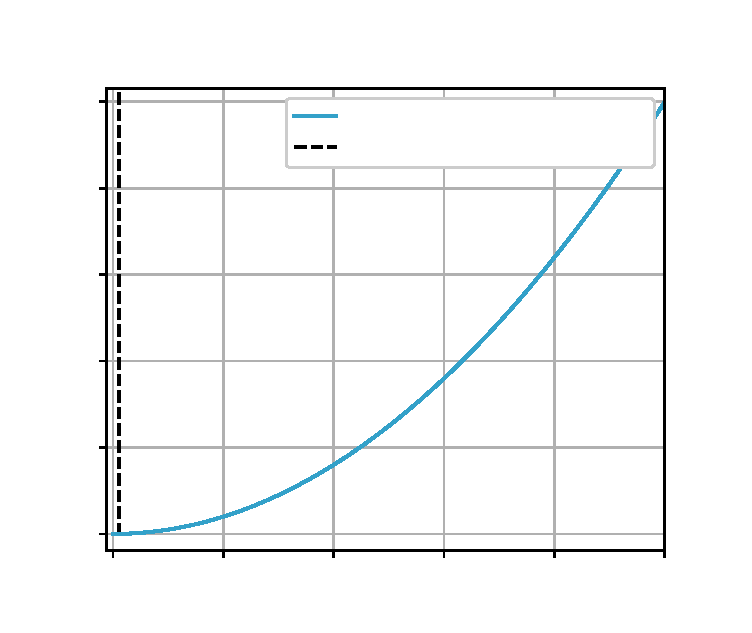
\includegraphics[width=\unitlength]{images_2ddl/eta.eps}}%
    \put(0.12494664,0.04955423){\color[rgb]{0,0,0}\makebox(0,0)[lb]{\smash{0}}}%
    \put(0.26935006,0.04955423){\color[rgb]{0,0,0}\makebox(0,0)[lb]{\smash{20}}}%
    \put(0.42297564,0.04955423){\color[rgb]{0,0,0}\makebox(0,0)[lb]{\smash{40}}}%
    \put(0.57660093,0.04955423){\color[rgb]{0,0,0}\makebox(0,0)[lb]{\smash{60}}}%
    \put(0.73022622,0.04955423){\color[rgb]{0,0,0}\makebox(0,0)[lb]{\smash{80}}}%
    \put(0.87462877,0.04955423){\color[rgb]{0,0,0}\makebox(0,0)[lb]{\smash{100}}}%
    \put(0.08654466,0.10358121){\color[rgb]{0,0,0}\makebox(0,0)[lb]{\smash{0}}}%
    \put(0.03121375,0.22391821){\color[rgb]{0,0,0}\makebox(0,0)[lb]{\smash{1000}}}%
    \put(0.03121375,0.34425464){\color[rgb]{0,0,0}\makebox(0,0)[lb]{\smash{2000}}}%
    \put(0.03121375,0.46459107){\color[rgb]{0,0,0}\makebox(0,0)[lb]{\smash{3000}}}%
    \put(0.03121375,0.58492749){\color[rgb]{0,0,0}\makebox(0,0)[lb]{\smash{4000}}}%
    \put(0.03121375,0.70526392){\color[rgb]{0,0,0}\makebox(0,0)[lb]{\smash{5000}}}%
    \put(0.46800464,0.68690835){\color[rgb]{0,0,0}\makebox(0,0)[lb]{\smash{$\eta_{max}$}}}%
    \put(0.46800464,0.64354118){\color[rgb]{0,0,0}\makebox(0,0)[lb]{\smash{\small valeur minimale de  $F/m_r g$ }}}%
    \put(0.46,0.0155423){\color[rgb]{0,0,0}\makebox(0,0)[lb]{\smash{$F/m_r g$}}}%
  \end{picture}%
\endgroup%

\caption{Variation de la hauteur maximale de saut adimensionnelle en fonction du ratio $F/m_r g$}
\label{fig:eta}
\end{figure}


\begin{figure}
\centering
\def\svgwidth{320}
%% Creator: Inkscape inkscape 0.92.2, www.inkscape.org
%% PDF/EPS/PS + LaTeX output extension by Johan Engelen, 2010
%% Accompanies image file 'eff.eps' (pdf, eps, ps)
%%
%% To include the image in your LaTeX document, write
%%   \input{<filename>.pdf_tex}
%%  instead of
%%   \includegraphics{<filename>.pdf}
%% To scale the image, write
%%   \def\svgwidth{<desired width>}
%%   \input{<filename>.pdf_tex}
%%  instead of
%%   \includegraphics[width=<desired width>]{<filename>.pdf}
%%
%% Images with a different path to the parent latex file can
%% be accessed with the `import' package (which may need to be
%% installed) using
%%   \usepackage{import}
%% in the preamble, and then including the image with
%%   \import{<path to file>}{<filename>.pdf_tex}
%% Alternatively, one can specify
%%   \graphicspath{{<path to file>/}}
%% 
%% For more information, please see info/svg-inkscape on CTAN:
%%   http://tug.ctan.org/tex-archive/info/svg-inkscape
%%
\begingroup%
  \makeatletter%
  \providecommand\color[2][]{%
    \errmessage{(Inkscape) Color is used for the text in Inkscape, but the package 'color.sty' is not loaded}%
    \renewcommand\color[2][]{}%
  }%
  \providecommand\transparent[1]{%
    \errmessage{(Inkscape) Transparency is used (non-zero) for the text in Inkscape, but the package 'transparent.sty' is not loaded}%
    \renewcommand\transparent[1]{}%
  }%
  \providecommand\rotatebox[2]{#2}%
  \ifx\svgwidth\undefined%
    \setlength{\unitlength}{344.79999138bp}%
    \ifx\svgscale\undefined%
      \relax%
    \else%
      \setlength{\unitlength}{\unitlength * \real{\svgscale}}%
    \fi%
  \else%
    \setlength{\unitlength}{\svgwidth}%
  \fi%
  \global\let\svgwidth\undefined%
  \global\let\svgscale\undefined%
  \makeatother%
  \begin{picture}(1,0.83526682)%
    \put(0,0){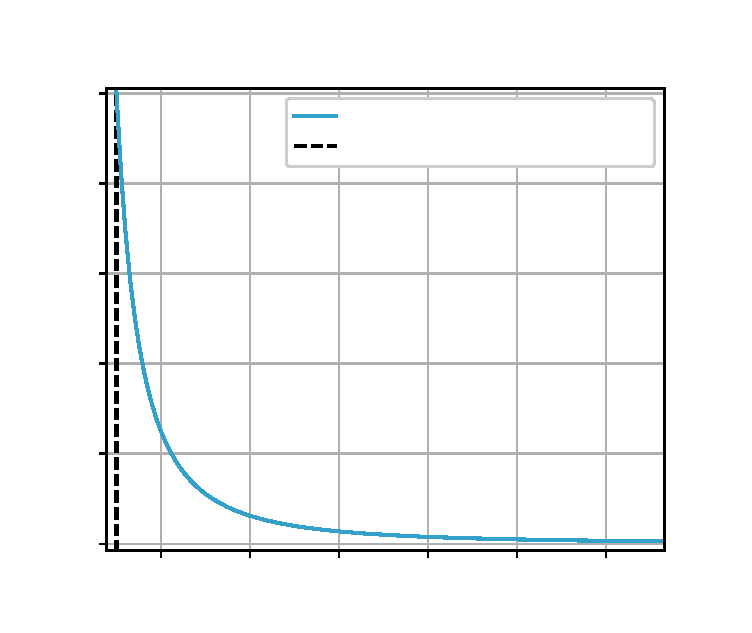
\includegraphics[width=\unitlength]{images_2ddl/eff.eps}}%
    \put(0.19169287,0.04955423){\color[rgb]{0,0,0}\makebox(0,0)[lb]{\smash{2}}}%
    \put(0.31560035,0.04955423){\color[rgb]{0,0,0}\makebox(0,0)[lb]{\smash{4}}}%
    \put(0.43950406,0.04955423){\color[rgb]{0,0,0}\makebox(0,0)[lb]{\smash{6}}}%
    \put(0.56341067,0.04955423){\color[rgb]{0,0,0}\makebox(0,0)[lb]{\smash{8}}}%
    \put(0.67809745,0.04955423){\color[rgb]{0,0,0}\makebox(0,0)[lb]{\smash{10}}}%
    \put(0.80200116,0.04955423){\color[rgb]{0,0,0}\makebox(0,0)[lb]{\smash{12}}}%
    \put(0.05885673,0.08975435){\color[rgb]{0,0,0}\makebox(0,0)[lb]{\smash{0.5}}}%
    \put(0.05885673,0.21525174){\color[rgb]{0,0,0}\makebox(0,0)[lb]{\smash{0.6}}}%
    \put(0.05885673,0.34074826){\color[rgb]{0,0,0}\makebox(0,0)[lb]{\smash{0.7}}}%
    \put(0.05885673,0.4662471){\color[rgb]{0,0,0}\makebox(0,0)[lb]{\smash{0.8}}}%
    \put(0.05885673,0.59174304){\color[rgb]{0,0,0}\makebox(0,0)[lb]{\smash{0.9}}}%
    \put(0.05885673,0.71724188){\color[rgb]{0,0,0}\makebox(0,0)[lb]{\smash{1.0}}}%
    \put(0.46800464,0.68690835){\color[rgb]{0,0,0}\makebox(0,0)[lb]{\smash{$E_{p,g}/E_{tot}$}}}%
    \put(0.46800464,0.64435615){\color[rgb]{0,0,0}\makebox(0,0)[lb]{\smash{\small valeur minimale de $F/m_r g$ }}}%
    \put(0.460200116,0.0155423){\color[rgb]{0,0,0}\makebox(0,0)[lb]{\smash{$F/m_r g$}}}%
  \end{picture}%
\endgroup%

\caption{Variation de l'efficacité énergétique en fonction du ratio $\dfrac{F}{m_r g}$}
\label{fig:effe}
\end{figure}


Remarques:
\begin{itemize}
    \item Les tracés adimensionnels permettent d'étudier une tendance globale, en s'affranchissant de la dépendance des résultats avec les autres paramètres.
    
\end{itemize}

